% !Tex root = ../main.tex

\chapter{新型数据结构}

在这一章,我们将重点介绍由布隆过滤器衍生出来的几个特殊数据结构,分别是布谷鸟过滤器,异或型过滤器以及不经意的键值存储。
% 从上一章的分类我们知道,对于

\section{布谷鸟过滤器}

从上一章的分类我们可以知道,布谷鸟过滤器是一种 OR 型的过滤器,且 $f(x)$ 为 $x$ 的指纹信息。
布谷鸟过滤器的概念最早是由 Fan 等人~\cite{fan2014cuckoo} 于2014年提出的,其构造方式受到了布谷鸟哈希表(Cuckoo Hash Table)~\cite{pagh2004cuckoo}的启发。
在介绍布谷鸟过滤器之前,我们首先介绍布谷鸟哈希表的构造。

\subsection{布谷鸟哈希表}

布谷鸟哈希表可以看作一个由多个桶(bucket)组成的数组结构。
对于每个元素 $x$ 来说,它在哈希表中对应两个候选位置,分别由两个哈希函数 $h_1(x)$ 和 $h_2(x)$ 决定。
在插入元素 $x$ 时,首先检查 $x$ 对应的两个位置上的桶中是否有多余位置。
如果两个桶都有多余空间,则直接将 $x$ 放入桶中;如果两个桶都已满,则随机在一个候选位置上踢出一个元素并将 $x$ 放入该位置上。踢出的元素则重新插入到它对应的另一个候选位置上。
如图所示,假设每个桶中都只能存储一个元素,当插入元素 $x$ 时,首先计算出它的两个候选位置分别是 $2$ 和 $6$。
因为 $2$ 和 $6$ 两个位置都已满,这里选择踢出位置 $6$ 上的元素 $a$,并将 $x$ 放入其中。
被踢出的 $a$ 则重新插入到它的另一个候选位置,也就是 $4$ 上。
由于位置 $4$ 上已有元素 $c$,则把 $c$ 踢出,将 $a$ 存储在位置 $4$ 中,并将 $c$ 重新插入到它的候选位置 $1$ 上,最终结果如图所示。
这种``踢出-插入''的思路与布谷鸟下蛋时会将蛋放入其他鸟的巢穴,并挤出原本巢中蛋的行为很相似,因此而得名。

\subsection{布谷鸟过滤器的构造}

与布谷鸟哈希表类似,布谷鸟过滤器也是由多个桶组成的数组结构。
不同的是,在布谷鸟过滤器中每个桶中存储的并不是元素本身,而是元素的指纹。
这就导致在将桶中的元素指纹踢出时,无法根据指纹信息确定它的另一个候选位置。
因此布谷鸟过滤器采用了部分密钥布谷鸟哈希(partial-key cuckoo hashing)的技巧来解决该问题。
也就是将元素的两个候选位置与元素的指纹值建立联系,这样就能在只知道元素的指纹值和其中一个位置信息的情况下计算出另一个位置信息。
具体来说,对于元素 $x$,其对应的两个候选位置计算如下:
\begin{align}
  h_1(x) & = \mathsf{hash}(x) \\
  h_2(x) & = h_1(x) \oplus \mathsf{hash}(x\mbox{'s fingerprint}) \label{eq:cuckoo_h2}
\end{align}
式~\ref{eq:cuckoo_h2}中的异或操作正好满足了上述性质,即$h_1(x)$ 也可以通过 $h_2(x)$ 和 $x$ 的指纹信息计算得出。
另外,在异或操作中采用的是$x$指纹的哈希而不是$x$的指纹本身,这样做是因为如果只用指纹本身的话,两个候选位置之间的距离就受限于指纹的取值范围。
比如使用 $8$ 比特长度的指纹,那么两个候选位置之间最多相差 $256$。
而使用指纹的哈希则可以确保两个候选位置可以分布在过滤器中的任意位置,从而降低哈希碰撞的概率并提高存储空间的利用率。

通过上述讨论,我们可以直接给出布谷鸟过滤器的 $\mathsf{Construct}$ 算法思路。
以输入集合 $S$ 为例,对于每一个元素 $x\in S$,插入 $x$ 的过程描述如下:
\begin{itemize}
  \item 首先计算 $x$ 的指纹值 $f$,以及两个候选位置信息 $h_1(x)$ 和 $h_2(x)$。
  \item 只要 $h_1(x)$ 和 $h_2(x)$ 两个位置上有一个桶有空余,那么直接将 $f$ 插入空余的桶中,否则进入下一步。
  \item 随机从 $h_1(x)$ 和 $h_2(x)$ 中选取一个位置 $i$,并从该位置上踢出一个指纹,并将 $f$ 插入。踢出的指纹再计算出它的另一个候选位置,执行插入步骤。
\end{itemize}
在布谷鸟过滤器的构造过程中,会设置一个最大踢出值,当踢出的指纹超过最大值时将直接返回错误指示符 $\perp$。

布谷鸟过滤器的 $\mathsf{Evaluate}$ 算法比较直接,给定输入的元素 $x$,只需要计算它对应的两个位置 $h_1(x)$ 和 $h_2(x)$,如果在这两个位置上至少有一个桶中含有 $x$ 的指纹,那么返回 $\mathsf{True}$,否则返回 $\mathsf{False}$。

除了在\textbf{定义~\ref{def:filter}}中的 $\mathsf{Construct}$ 和 $\mathsf{Evaluate}$ 两个算法之外,布谷鸟过滤器中还支持删除操作。
这也是布谷鸟过滤器相比布隆过滤器的一大优势。
删除算法与 $\mathsf{Evaluate}$ 算法类似,也比较直接,即对需要删除的元素 $x$ 计算出 $h_1(x)$ 和 $h_2(x)$ 两个位置之后,如果这两个位置上有一个包含 $x$ 的指纹,则直接移除该位置上的指纹信息。
注意在删除过程中,如果找到两个位置上都存在 $x$ 的指纹时,只需要移除其中一个位置上的指纹信息即可。
这是因为当两个元素具有相同的指纹信息时,这样做就不会影响对另一个元素的存在性判断。
当然,只删除一个会带来假正例的问题,但这对于大部分过滤器结构来说都是无法避免的,我们只需要将假正例的概率控制在较小的值即可。

\subsection{布谷鸟过滤器的性能}

我们用 $|f|$ 表示指纹值的比特长度,当给定 $h_1(x)$ 的值时,也就确定了 $h_2(x)$ 有 $2^{|f|}$ 种不同取值。
假设布谷鸟过滤器中包含 $m$ 个桶,当 $2^{|f|} < m$ 时,$h_2(x)$ 的取值范围也就是整个过滤器长度的子集。
因此,当 $|f|$ 取值越小时,哈希碰撞的几率也会越大,构建过滤器的失败概率也会随之增大。
而且当 $m$ 与 $2^{|f|}$ 之间的差距越大时,布谷鸟过滤器的空间利用率也会越低。
% $m$ 与 $2^|f|$ 的差距越大时,哈希碰撞的几率
如何设定合适的参数就显得尤为重要。

% 假定有 $q$ 个元素对应相同位置的两个桶,其中第一个元素 $x$ 对应的第一个位置为 $h_1(x)$,其指纹信息为 $t_x$。
% 那么其他 $q-1$ 个元素必须满足:1)具有相同的指纹 $t_x$,即概率为 $1/2^{|f|}$;2)具有相同的位置 $h_1(x)$ 或 $h_1 \oplus h(t_x)$,即概率为 $2/m$。
% 因此 $q$ 个元素共享相同位置的概率为 $(2/m \cdot 1/2^{|f|})^{q-1}$。

我们用负载因子 $\alpha$ ($0\leq \alpha \leq 1$) 来表示布谷鸟过滤器的空间利用率,它的定义是过滤器中已占用空间大小与过滤器大小的比值。
因此当 $\alpha$ 的值越接近 $1$,那就表示空间利用率越高。
% 从文献~\cite{fan2014cuckoo}的实验结果来看,当
在给定指纹长度 $|f|$ 和负载因子 $\alpha$ 的情况下,对于每个元素均摊的空间开销 $C$ 可以表示为:
\begin{equation}
  C = \frac{\mbox{过滤器的存储大小}}{\mbox{存储的条目数}} = \frac{|f| \cdot \mbox{总条目数}}{\alpha \cdot \mbox{总条目数}} = \frac{|f|}{\alpha} \mbox{ bits}.
  \label{eq:cuckoo_C}
\end{equation}
负载因子的大小受到桶大小(用 $b$ 表示)的影响。
当 $b=1$ 时,负载因子仅有 $50\%$,而当 $b=4$ 或 $b=8$ 时,负载因子随之增长为 $95\%$ 和 $98\%$。
而当桶越大时,就越容易出现碰撞(即相同指纹信息)的情况。
为了保证相同的假正例概率,就要求指纹长度越长。
根据文献~\cite{fan2014cuckoo}中的推导,指纹长度 $|f|$ 与假正例率 $\epsilon$ 和桶大小$b$ 之间的关系如下所示:
\begin{equation}
  |f| \geq \lceil\log_2(2b / \epsilon) \rceil = \lceil \log_2(1/\epsilon) + \log_2(2b) \rceil \mbox{ bits}.
  \label{eq:cuckoo_f}
\end{equation}
从式~\ref{eq:cuckoo_C}和式~\ref{eq:cuckoo_f}可以得出:
\begin{equation}
  C \leq \lceil \log_2(1/\epsilon) + \log_2(2b) \rceil / \alpha.
  \label{eq:cuckoo_storage}
\end{equation}
当 $b=4$ 时,此时均摊空间开销约为 $(\log_2(1/\epsilon) + 3) / \alpha$,其中 $\alpha \approx 95\%$。
而对于布隆过滤器,其均摊空间开销约为 $1.44 \log_2(1/ \epsilon)$。
因此,相比于布隆过滤器,布谷鸟过滤器可以实现更优的均摊空间开销。
文献~\cite{fan2014cuckoo}中的实验结果表示,当 $b$ 取 $4$ 的时候,布谷鸟过滤器能在假正例率和空间开销之间取得较好的平衡。

% 我们使用 $b$ 来表示桶的大小。
% 当哈希函数数量为 $2$,$b=1$ 时,负载因子 $\alpha$ 为 $50\%$。
% 但当我们增加 $b$ 的大小时,负载因子会随之增长。

\subsection{布谷鸟过滤器的优化}

% 排序进行优化

\section{异或型过滤器}

Bloomier 过滤器~\cite{chazelle2004bloomier,charles2008bloomier} 是首个异或型结构的过滤器。
与前面介绍的布隆过滤器和布谷鸟过滤器不同,它并不是用来判断元素是否属于某一集合,而是用来返回元素对应函数值的一种概率型数据结构。
从这一角度来看,Bloomier 过滤器的定义更接近于不经意的键值存储(即\textbf{定义~\ref{def:okvs}})而非过滤器(即\textbf{定义~\ref{def:filter}})。
由于 Bloomier 过滤器不关注其存储的函数 $f(x)$ 是如何定义的,它也被看作是其他过滤器的一种一般化形式~\cite{graf2020xor,li2023chainedfilter}。
严格来说,Bloomier 过滤器的定义与不经意的键值存储还是不同,因为在不经意的键值存储中,要求对于任意 $x'\notin S$ 均返回一个随机结果,但 Bloomier 过滤器要求大概率返回 $\perp$。
为了叙述上的统一,本文还是将 Bloomier 过滤器归类为过滤器而非不经意的键值存储。

早期的 Bloomier 过滤器~\cite{chazelle2004bloomier} 采用的是两个哈希表的构造。
对于给定的元素集合 $S= \{x_1, x_2, \dots, x_n\}$,Bloomier 过滤器为集合中每一个元素 $x_i$ 通过哈希函数计算出一组位置信息 $\{h_1(x_i), h_2(x_i), \dots, h_k(x_i)\}$,并通过贪心算法确定出与其他元素均不冲突的位置 $\tau(x_i)$。
然后将该位置信息的编码通过异或拆分并记录在第一个哈希表$\mathsf{T}_1$ 的各个位置 $\{h_1(x_i), h_2(x_i), \dots, h_k(x_i)\}$ 上,将 $f(x)$ 的结果存储在第二个哈希表 $\mathsf{T}_2$ 的位置 $\tau(x_i)$ 上。
判断时,以输入 $x_i$ 为例,Bloomier 过滤器首先计算出对应的位置信息 $\{h_1(x_i), \dots, x_n\}$,然后通过将 $\mathsf{T}_1$ 上这些位置上对应的值进行异或得到 $\tau(x_i)$ 的编码。
如果解码后得到的结果在 $\mathsf{T}_2$ 长度范围内,则直接返回所在位置的结果,否则返回 $\perp$。
因为该构造需要使用两个哈希表进行存储,且构造需要使用贪心算法,无论在存储方面还是在构建过程中都存在较大的开销。
% 因为该构造需要使用贪心算法找出非冲突地址,构建
% 且使用两个哈希表存储所占用的存储开销也比较大,
后续的工作~\cite{charles2008bloomier}通过组建方程的形式,将构建复杂度从原本的 $O(n\log(n))$ 降低为 $\log(n)$。
但这些工作为了确保返回的是 $f(x)$,需要在增加额外的信息用于判断 $x'\notin S$ 的情况,在构建效率和存储开销上都不能进一步提高。
% 下面将介绍的异或型过滤器
后续的异或型过滤器~\cite{graf2020xor,dillinger2021ribbon,graf2022binary}继承了 Bloomier 过滤器中异或操作的思路,但它们只考虑做元素是否属于某一集合的判断,并不考虑返回 $f(x)$ 本身。
这些过滤器无论在构建上还是在存储开销上都相比 Bloomier 过滤器有极大的提升,以下我们将对它们进行逐一介绍。

% 在两个哈希表中,Bloomier
% 通过贪心算法为集合中的每一个元素 $x_i$ 确定一个与其他元素均不冲突的位置 $\tau(x_i)$,然后将

% 简单介绍 Bloomier 过滤器定义,与一般性定义的区别,与 OKVS 的区别;
% Bloomier 过滤器与 second look 的构造,以及复杂度

% 1. 但在很长一段时间内,没有较为高效的构造算法。
% 2. 直到 异或过滤器和

\subsection{异或过滤器}

% 构造关键在与如何确定唯一不冲突的位置

首先介绍异或过滤器(Xor filter)~\cite{graf2020xor}。
% 正如表~\ref{tab:construct}中所示,异或过滤器
正如前面所说,异或过滤器继承了 Bloomier 过滤器中异或操作的思想,但它返回的并不是 $f(x)$,而是判断 $x$ 是否属于集合 $S$,即符合\textbf{定义~\ref{def:filter}}中的描述。
% 异或过滤器的构造受到
异或过滤器的 $\mathsf{Construct}$ 过程包含以下步骤:
\begin{itemize}
  \item 首先选择一个长度为 $\approx 1.23n$ 的数组,并将数组划分成三个相等的区域,即每个区域长度为 $\approx 1.23n/3$。
  \item 使用三个哈希函数计算出每个元素对应三个区域上的位置。
  \item 在确定所有元素的位置之后,我们开始统计数组中每一个位置上对应的元素个数。如果找到某个位置上只存在一个元素,那么将该元素压入栈中,并将该元素在数组上的信息全部移除。
每次移除一个元素,数组中就有可能出现新的只存在一个元素的位置。
  \item 循环上一步骤,直到所有元素都压入栈中,否则构建失败,返回 $\perp$。
  \item 最后只需要将元素从栈中逐个取出,计算该元素对应的三个位置,并将元素对应的指纹信息通过异或拆分成三份放入这三个位置。
\end{itemize}
% 要构建异或过滤器,
% 循环此过程直到所有的元素都压入栈中。
% 并将每个元素对应的指纹通过
按照这样的移除方式,对于每个出栈的元素,可以确保至少有一个位置上为空。
因此可以通过为该位置计算出特殊的取值,确保元素对应所有位置上的异或结果正好是其指纹值。
以元素 $x_i$ 为例,假如它的三个位置分别为 $h_1(x_i)$,$h_2(x_i)$ 和 $h_3(x_i)$,需要构建的数组为 $F$,且 $F[h_3(x_i)]$ 上为空,其它两个位置上已有信息,那么可以通过以下方式进行计算:
\begin{equation}
  F[h_3(x_i)] = f(x_i) \oplus F[h_1(x_i)] \oplus F[h_2(x_i)].
\end{equation}
这里 $f(x_i)$ 表示为 $x_i$ 的指纹值。
这样计算也就是为了让 $x_i$ 在 $F$ 上对应三个位置上的值异或后的结果为 $f(x_i)$。

在理解了异或过滤器的构造之后,它的判断过程也就非常直接。
对于任意给定元素 $x_i$,其 $\mathsf{Evaluate}$ 过程如下:
\begin{itemize}
  \item 首先通过哈希函数计算出它的三个位置信息 $h_1(x_i)$,$h_2(x_i)$ 和 $h_3(x_i)$。
  \item 将这三个位置上对应的值进行异或,得到 $v = h_1(x_i) \oplus h_2(x_i) \oplus h_3(x_i)$。
  \item 如果 $v$ 与 $f(x)$ 相等,那么返回 $\mathsf{True}$,否则返回 $\mathsf{False}$。
\end{itemize}

异或过滤器出现假正例的情况就是出现 $x'\notin S$ 且 $\mathsf{Evaluate}$ 结果正好等于 $x'$ 的指纹。
也就是说异或过滤器的假正例率与指纹长度有关。
假设指纹长度为 $|f(x)|$,那么假正例率 $\epsilon = 1 / 2^|f(x)|$。
当集合非常大时,异或过滤器构造成功的概率可以达到 $100\%$。
比如当集合大小为 $10^7$ 时,构建成功的概率几乎为 $1$。
对于小集合,文献~\cite{graf2020xor}通过实验发现,当过滤器长度设定为 $1.23 n + 32$ 时,成功构建的概率要大于 $0.8$。
% 的假正例率与指纹长度有关,
% 异或过滤器的构造思路受到

% 从异或过滤器的构造过程可以得出,它在构建时
相比布谷鸟过滤器,异或过滤器具有更低的存储开销。
为了分析异或过滤器的空间性能,我们还是用 $\alpha$ 表示异或过滤器的负载因子。
当过滤器长度设定为 $1.23n + 32$ 时,$\alpha$ 大约为 $0.81$。
在给定指纹长度 $f(x)$ 与负载因子 $\alpha$ 之后,我们可以得到每个元素均摊的空间开销 $C$ 为
\begin{equation}
  C = \frac{\mbox{过滤器存储大小}}{\mbox{集合元素的数量}} = \frac{|f(x)| \cdot \mbox{过滤器条目数}}{\alpha \cdot \mbox{过滤器条目数}} = \frac{|f(x)|}{\alpha} = \frac{\log_2(1/\epsilon)}{\alpha} \mbox{ bits}.
  \label{eq:xor_storage}
\end{equation}
从式~\ref{eq:xor_storage}和式~\ref{eq:cuckoo_storage}可以看出,当指纹长度和负载因子相同时,异或过滤器的均摊空间要比布谷鸟过滤器更低。
在实际中,由于两个过滤器在构造方法上完全不同,它们的负载因子也不能取到相同的结果。
比如在布谷鸟过滤器中,负载因子 $\alpha$ 与桶的长度密切相关,$b=1$ 时,$\alpha$ 仅为 $50\%$,当 $b=4$ 时,$\alpha$ 可以达到 $95\%$。
而在异或过滤器中,理想情况下过滤器长度设定为 $1.23n + 32$,即 $\alpha$ 为 $81\%$。
尽管异或过滤器并不能像布谷鸟过滤器那样可以调节 $\alpha$ 的值,但考虑到布谷鸟过滤器是通过扩大桶的容量来增大 $\alpha$ 的值,其均摊存储开销会随着桶的容量增加而增加。
就整体均摊存储开销而言,异或过滤器还是要优于布谷鸟过滤器。


相比Bloomier 过滤器~\cite{chazelle2004bloomier},异或过滤器在构建上更为高效。
因为异或过滤器在构造时并不需要使用贪心算法来计算互不冲突的位置,而是直接对元素进行按序扫描,复杂度只与集合元素数量有关。
在存储开销方面,异或过滤器由于只需要使用一个哈希表直接记录,相比 Bloomier 过滤器采用的两个哈希表的方式所需存储空间更小。

\subsection{二进制引信过滤器}

尽管异或过滤器在存储开销方面要优于布隆过滤器和布谷鸟过滤器,但它还存在优化的空间。
2022 年,异或过滤器的作者 Graf 和 Lemire 在之前的基础上提出了一种新的异或型过滤器,称为二进制引信过滤器(Binary Fuse Filter)~\cite{graf2022binary}。
相比异或过滤器,二进制引信过滤器将存储开销降低了$10\%$ 到 $15\%$。
而做到这一点仅仅只需要修改哈希函数的映射方式。
% 最初使用哈希函数映射位置的方式。

二进制引信过滤器根据使用的哈希函数数量不同又分为3-wise 二进制引信过滤器和 4-wise 二进制引信过滤器,前者使用 3 个哈希函数,后者使用 $4$ 个哈希函数。
这里为了方便介绍以及与异或过滤器进行对比,我们默认哈希函数数量为 $3$。
二进制引信过滤器的构造与异或过滤器类似,其 $\mathsf{Construct}$ 过程描述如下:
\begin{itemize}
  \item 首先选择一个长度为 $\approx 1.125 n$ 的数组,并将它划分成若干个区域,每个区域长度为 $2^{\lfloor \log_{3.33}n + 2.25\rfloor}$。
  \item 使用三个哈希函数计算出每个元素对应的三个位置。这里要求三个哈希函数映射的三个位置所在区域为连续的三个区域。
  \item 根据第一个哈希函数映射的位置对元素进行排序,这样一来,第一个元素就应该被映射到前三个区域。按照排序后的顺序,逐个寻找只有一个元素的位置。如果找到,就将该元素压入栈中,并将该元素在数组中的所有信息全部移除。每次移除一个元素,数组中就有可能出现新的只存在一个元素的位置。
  \item 循环上一步骤,直到所有元素都压入栈中,否则构建失败,返回 $\perp$。
  \item 最后只需要将元素从栈中逐个取出,计算该元素对应的三个位置,并将元素对应的指纹信息通过异或拆分成三份放入这三个位置。
\end{itemize}
从构建过程来看,二进制引信过滤器与异或过滤器非常相似。
二者主要在映射方式上有所区别。
在异或过滤器中,首先会将数组分成三个长度相同的区域,然后使用三个哈希函数将元素映射到这三个区域。
而在二进制引信过滤器中,将数组分成的就不是三个区域,而是若干个长度为 $2^{\lfloor \log_{3.33}n + 2.25\rfloor}$ 的区域。
在使用哈希函数映射时,要求得到的三个位置对应连续的三个不同区域。
仅仅通过调整了哈希函数的映射方式,二进制引信过滤器就能将构造的数组长度从异或过滤器的 $1.23n$ 压缩到 $1.125n$。

二进制引信过滤器的 $\mathsf{Evaluate}$ 过程与异或过滤器很类似,也是通过计算三个位置信息,再将数组中这三个位置上的值进行异或,得到结果与所输入的元素指纹做对比,如果相等则返回 $\mathsf{True}$,否则返回 $\mathsf{False}$。

与异或过滤器相同,二进制引信过滤器均摊空间开销 $C$ 也是与假正例率 $\epsilon$ 和负载因子 $\alpha$ 有关,即
\begin{equation}
  C = \frac{|f(x)|}{\alpha} = \frac{\log_2(1/ \epsilon)}{\alpha}.
\end{equation}
但因为二进制引信过滤器采用不同的映射方式,其负载因子 $\alpha$ 要比异或过滤器更大,也就是说当二者指纹函数长度相同时,二进制引信过滤器的均摊开销要比异或过滤器更低。
二进制引信过滤器的负载因子取决于使用的哈希函数数量。
当使用三个哈希函数时,负载因子理论上大约为 $88\%$,而当使用四个哈希函数时,负载因子可以提升到 $93\%$。
文献~\cite{graf2022binary}给出了数组长度和每个区域大小的参考公式,如表~\ref{tab:binary_fuse_filter}所示。
\begin{table}
  \centering
  \caption{不同哈希函数数量情况下的参数设置}
  \label{tab:binary_fuse_filter}
  \begin{tabular}{ccc}
    \toprule
    过滤器类型  &  数组长度  &  每个区域大小  \\
    \midrule
     3-wise &  $\left\lfloor \left(0.875 + 0.25 \max\left(1, \frac{\log10^6}{\log n}\right)\right) n \right\rfloor \geq \left\lfloor 1.125n \right\rfloor$  &  $2^{\lfloor \log_{3.33}n + 2.25 \rfloor} \approx 4.8 \cdot n^{0.58}$  \\
     4-wise &  $\left\lfloor \left(0.77 + 0.305 \max \left(1, \frac{\log(6\cdot 10^5)}{\log n}\right)\right) n \right\rfloor \geq \left\lfloor 1.075 n \right\rfloor$  & $2^{\lfloor \log_{2.91}n - 0.5 \rfloor} \approx 0.7\cdot n^{0.65}$  \\
    \bottomrule
  \end{tabular}
\end{table}

\subsection{缎带过滤器}

% 当二进制引信过滤器通过调整哈希函数映射方式来进一步压缩异或过滤器的存储开销,
在二进制引信过滤器提出的几乎同一时间,还有另一个独立工作~\cite{dillinger2021ribbon}提出了比异或过滤器更优的异或型过滤器,名为缎带过滤器(Ribbon Filter)。
与异或过滤器及二进制引信过滤器不同,缎带过滤器通过求解方程组的形式来完成过滤器的构造。
这里我们使用 $Z$ 来表示缎带过滤器构造的数组,假设其长度为 $m$,即此时的负载因子为 $\alpha = n / m$。
我们将数组看作 $m$ 长度的向量,假设指纹长度为 $r$,那么 $Z$ 就可以看作是 $m\times r$ 的比特矩阵,即 $Z \in \{0,1\}^{m\times r}$。
对于每个元素 $x_i$,假设存在一个哈希函数 $h$ 使得 $h(x)$ 的长度为 $m$ 比特。
我们只需要构造这样的 $Z$,使得对于集合 $S$ 中的每一个元素 $x_i$ 都有 $h(x_i) \cdot Z = f(x_i)$ 成立。
这样 $\mathsf{Evaluate}$ 也就可以看作计算内积 $h(x_i) \cdot Z$ 并比对结果是否为 $f(x_i)$ 的过程。
% 这种构造困难的地方在于如何构造
因此,目前最大的问题就是如何构造这样的 $Z$,该问题的根本在于哈希函数 $h$ 应该如何设计。

受到文献~\cite{dietzfelbinger2019Efficient}中所构造的快速高斯消元法的启发,缎带过滤器将哈希函数 $h$ 的计算分为两个部分。
% 缎带过滤器参考了文献~\cite{dietzfelbinger2019Efficient},
首先需要设定一个小于 $m$ 的参数 $w$,$w$ 也被称为缎带宽度 (ribbon width)。
对于给定的元素 $x$,$h(x)$ 的值取决于一个随机起始位置 $s(x)\in [m-w-1]$ 和一个长度为 $w$ 比特的随机系数向量 $c(x) \in \{0,1\}^w$。
在给定这两个值之后,哈希函数 $h(x)$ 的形式为:
\begin{equation}
  h(x) = 0^{s-1}c(x)0^{m-s-w+1}.
\end{equation}
与文献~\cite{dillinger2021ribbon}不同,在缎带过滤器的构造中,需要强制将 $c(x)$ 的第一个比特设为 $1$\footnote{作者表示这样的改变并不会影响解方程的效率,在分析时还是假设 $c(x)$ 为 $\{0,1\}^w$ 上的均匀分布~\cite{dillinger2021ribbon}。}。
在 $\mathsf{Construct}$ 过程中,缎带过滤器需要构造形如 $M \cdot Z = B$ 的方程组,其中 $M$ 为 $m\times m$ 的矩阵,$B$ 为 $m\times r$ 的矩阵。最终求解得到的 $Z$ 就是所构建的过滤器。
我们用 $M[i]$ 表示矩阵 $M$ 的第 $i$ 行,在构建之前,缎带过滤器需要初始化全为 $0$ 的 $M$ 和 $B$ 两个矩阵。
对于集合 $S$ 中的每一个元素 $x$,缎带过滤器中 $M$ 和 $B$ 的构造过程如下:
% $\mathsf{Construct}$ 过程描述如下:
\begin{itemize}
  \item 根据 $x$ 计算其起始位置 $i\gets s(x)$,哈希函数结果 $c \gets h(x)$,以及指纹函数结果 $b \gets f(x)$。
  \item 如果 $M[i]$ 为 $0^{m}$,则直接将令 $M[i] \gets c$,$B[i] \gets c$,并返回插入成功。否则,计算 $c \gets c \oplus M[i]$,$b \gets b \oplus B[i]$。
  \item 当 $c=0^{m}$ 且 $b = 0^{m}$ 时,返回重复插入;当 $c=0^{m}$ 但 $b \neq 0^{m}$ 时,返回插入失败;当 $c\neq 0^{m}$ 时,找到 $c$ 上第一个比特为 $1$ 的位置,记为 $i$,并返回上一步继续执行。
\end{itemize}
这里唯一出现插入失败的情况是当 $c=0^{m}$ 但 $b\neq 0^{m}$ 时,换句话说,在这种情况下两个元素产生了哈希碰撞但又具有不同的指纹结果,这样就会导致方程无解,从而导致插入元素失败。
% 这种情况的解决方法就是增大 $m$ 的值,尽量避免
当集合 $S$ 中所有元素都成功插入,则开始对方程组 $M \cdot Z = B$ 进行求解,得到的 $Z$ 便是所构建的过滤器。
从以上过程也可以发现,这样所构建的矩阵 $M$ 为一个近似于三角矩阵的形式,如图~\ref{fig:ribbon_construc}所示,因此可以直接使用向后替换法来快速对方程求解。

\begin{figure}[ht]
  \centering
  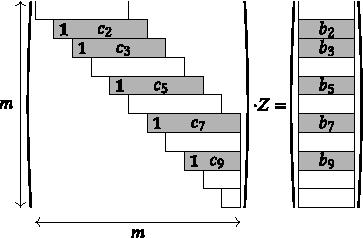
\includegraphics[width=0.8\textwidth]{figures/ribbon_filter_construction.pdf}
  \caption{缎带过滤器构造过程中的矩阵示例(来源:文献~\cite{dillinger2021ribbon})}
  \label{fig:ribbon_construc}
\end{figure}

缎带过滤器的 $\mathsf{Evaluate}$ 过程就比较直接,对于给定的输入 $x$,只需要计算 $h(x)\cdot Z$ 的结果是否与 $f(x)$ 相等即可。
因为方程中所有元素都是使用二进制形式来表示,实际上这一过程就是将 $h(x)$ 中所有为 $1$ 的位置对应在 $Z$ 上的值进行异或,如式~\ref{eq:ribbon_query}所示。
而异或过滤器和二进制引信过滤器在 $\mathsf{Evaluate}$ 也是类似的方式,只不过它们只需要找到三个(或四个)位置上的值进行异或。
但考虑到异或操作本身执行效率非常高,缎带过滤器虽然需要处理更多的异或操作,但实际中这些差距并不明显。
\begin{equation}
  h(x) \cdot Z = \bigoplus Z[i] \mbox{, } \forall i \in h(x) \mbox{ and } h(x)[i] = 1.
  \label{eq:ribbon_query}
\end{equation}

缎带过滤器的原文~\cite{dillinger2021ribbon}并没有给出理论上的存储开销分析,而是通过一系列实验验证缎带过滤器在存储上的优势。
而实验中主要是将异或过滤器和缎带过滤器的两个扩展版本进行对比,这两个扩展版本分别是齐次缎带过滤器(Homogeneous Ribbon filter)和平衡缎带过滤器(Balanced Ribbon filter)。
% 对比的是缎带过滤器的两个扩展版本
% 文献~\cite{dillinger2021ribbon}中还对缎带过滤器提出了两个扩展版本,分别是。
从实验结果来看,在相同的假正例率情况下,随着哈希函数中的参数 $w$ 越大,负载因子也随之增大。
当 $w=32$,$\epsilon=2^{-8}$ 时,齐次缎带过滤器的负载因子与异或过滤器相当。
而对于平衡缎带过滤器,当 $w$ 分别取 $32$ 和 $64$ 时,其负载因子可以达到 $96\%$ 甚至 $99\%$。


异或过滤器和二进制引信过滤器中的哈希函数可以看作映射为只有三个位置为 $1$ 比特其他位置都为 $0$ 形式。
这种哈希函数在之前的工作~\cite{botelho2013Practical,genuzio2016Fast}中实际也有讨论。

\section{不经意键值存储}

不经意键值存储(Obilivious Key-Value Store,OKVS)的概念最早是由 Garimella 等人~\cite{garimella2021oblivious}于2021年提出的。
正如\textbf{定义~\ref{def:okvs}}中所述,不经意键值存储包含 $\mathsf{Encode}$ 和 $\mathsf{Decode}$ 两个算法,它主要对键值型数据进行编码。
% OKVS 针对的是键值型数据,
对于编码结果 $D$,当其存储的键值对 $\{k, v\}$ 中 $v$ 为随机的数值,那么 $D$ 会隐藏关于 $k$ 的信息。
这也就是所谓的不经意性。

最直接的构造方式是多项式插值法,也就是说对于 $k_i \mapsto v_i$ 的映射看作坐标 $(k_i, v_i)$,通过插值构造多项式 $p$,使得 $p(k_i) = v_i$ 成立。
% 即把键值型数据 $\{(k_1, v_1), (k_2, v_2), \dots, (k_i, v_i), \dots (k_n, v_n)\}$ 中的 $(k_i, v_i)$ 看作坐标,通过插值确定多项式 $p$,使得对于 $(k_i, v_i)$ 满足 $p(k_i) = v_i$。
对于编码我们只需要记录多项式的系数,而系数个数刚好就是插值的坐标数量,因此这种构造方式的负载因子刚好为 $1$。
尽管在存储方面达到最优,但采用多项式插值的方式在编码时需要 $O(n\log^2n)$ 的复杂度~\cite{moenck1972Fast},当编码的键值对数量太大时,编码开销较大。
这就需要构造在存储和编解码开销之间取平衡的构造。

\subsection{构造思路}



\subsection{RB-OKVS}

\section{总结}
